\documentclass[a4paper,titlepage,oneside]{article}
\author{Ronan Legardinier}
\title{Graphics library selection}
\date{\today{}}
\usepackage[french]{babel}
\usepackage[utf8]{inputenc}
\usepackage{graphicx}

\begin{document}
	\maketitle{}
	\newpage
	
	\tableofcontents{}
	\newpage
	
	\section{Context}
		Vilain:: project. Choice of graphic library to GUI development.
	\section{Needs}
	
		Vilain:: GUI require graphics elements like value selectors, tabs, selectable lists, checkboxes, undraggable panels and a monitoring space.
	\section{Constraints}
		Vilain:: GUI needs 
	\section{Possible solutions}
		We have two solution of library:
			\paragraph{ofxGui}
				\begin{center}
					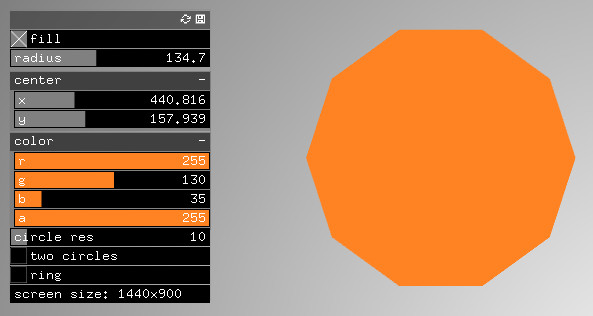
\includegraphics[width=400pt]{../Images/ofxGui.jpg}
					Screenshot 1 - Gui example with ofxGUI
				\end{center}
				
			\newpage
			
			\paragraph{ofxUi}
				\begin{center}
					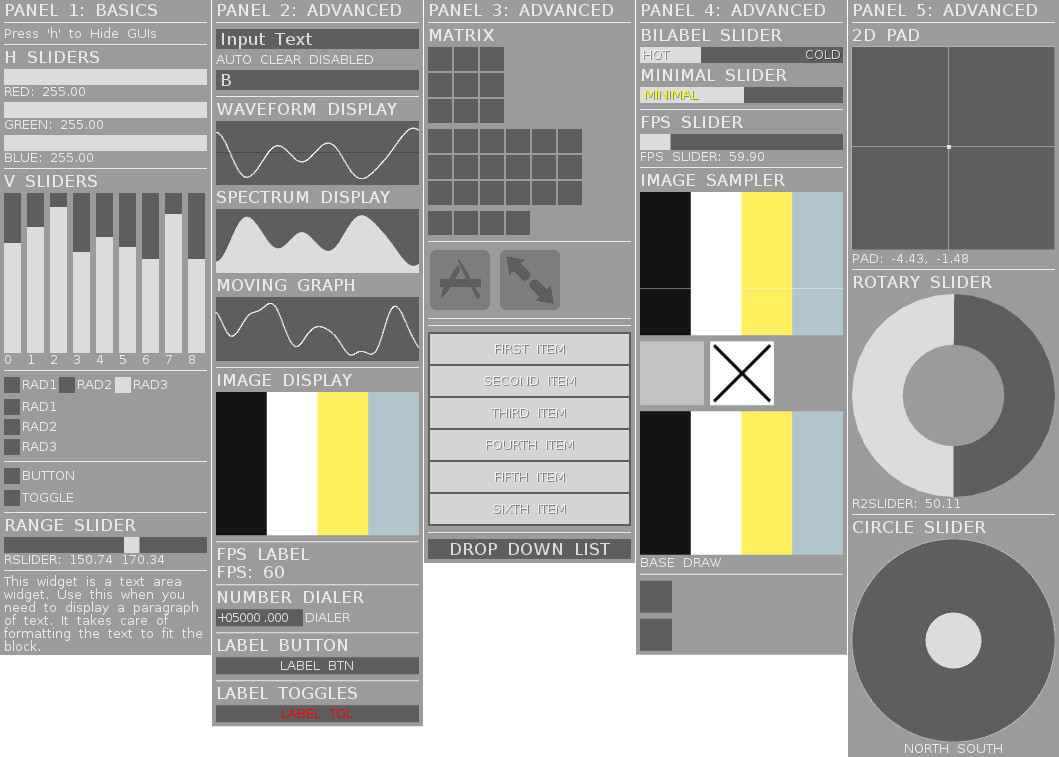
\includegraphics[width=400pt]{../Images/ofxUI.jpg}
					Screenshot 2 - Gui example with ofxUI
				\end{center}
								
	\section{Comparison / Selection}
		\begin{tabular}{ l || c | r }
			Critères & ofxGUI & ofxUI \\
		\end{tabular}\\
		ofxUI seems to be better than ofxUI due to the number of graphics elements it offers, particularly those needed for the project.
	\section{Implementation example}
	
\end{document}
